\section{Background}
\subsection{Hanabi}

The Hanabi Challenge has become a popular benchmark in MARL due to its unique properties as a cooperative, partially observable game where players must deduce each other's intentions to succeed. Unlike many competitive MARL tasks, Hanabi requires long-term strategies and implicit communication, posing unique challenges for traditional and deep reinforcement learning algorithms.
\paragraph*{Gameplay}
Hanabi is a cooperative card game of two to five players working together to achieve a common goal. It is often described as a form of cooperative solitaire. The game is played with a deck of cards, each with a colour and a number. The game's goal is to play cards in ascending order for each colour, starting from 1 to 5. Players can only see the cards of other players but have to infer the cards in their hands from the actions of other players. Players can give hints to each other about the cards in their hands, but they are limited in the number of hints they can give, they can also play cards but lose a life if they play a card incorrectly, and they can discard cards to gain more hints.
The game ends when the deck is empty, or the number of incorrect plays reaches a certain threshold. The players' score is determined by the number of cards played correctly by the end of the game, or 0 if the game ends due to too many incorrect plays.

\begin{figure}[h]
    \centering
    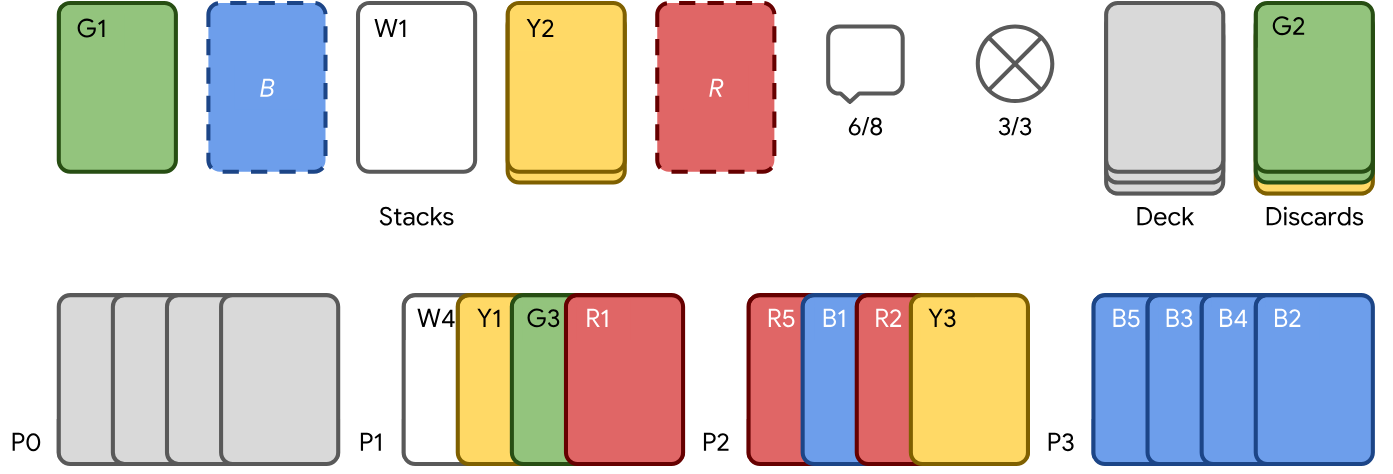
\includegraphics[width=\linewidth]{images/Hanabi.png}
    \caption{
      Four player Hanabi gameplay from the perspective of Player 0. The player can see the cards of other players but not their own, and the goal is to play cards in ascending order for each colour. This image is taken from the Hanabi Challenge paper \cite{bardHanabiChallengeNew2020a}
    }
    \Description{Training curve for Rainbow Agent}
  \end{figure}

\paragraph*{Challenges}
Hanabi was first presented as a challenge for AI research as early as 2015 by \textcite{osawaSolvingHanabiEstimating2015} to serve as a benchmark for evaluating the imitation of human intelligence with artificial intelligence. The work showcased strategies that attempted to recognize intent and infer hidden information to achieve high scores in Hanabi. The first rule-based approaches appeared later that year by \textcite{coxHowMakePerfect2015}. Since then, several deep-reinforcement learning algorithms have been developed to play Hanabi, achieving superhuman performance \cite{huSimplifiedActionDecoder2021, canaanEvaluatingRlAgents2020, foersterBayesianActionDecoder2019}.
Hanabi presents several challenges for MARL algorithms. The game is partially observable, meaning that players can only see the cards of other players and have to infer the cards in their hands from the actions of other players. This requires agents to develop theory-of-mind reasoning to infer the intentions of other players. The game also requires long-term planning and coordination between players, as the actions of one player affect the actions of other players. Finally, the game is stochastic, as the deck is shuffled at the beginning of each game, and the actions of other players can be unpredictable.
\textcite{bardHanabiChallengeNew2020a} identified several key areas to focus on when developing agents for Hanabi. The need for sample efficient deep reinforcement learning algorithms that can learn to coordinate in Hanabi's complex environment, which, despite its relatively small state and action space, is challenging due to the partially observable and cooperative nature of the game. Additionally, the ability of agents to cooperate effectively with themselves, otherwise known as self-play, is also a key area of focus. Finally, the ability of agents to generalize and adapt to new partners is also a key area of focus, as agents need to adapt to different play styles and strategies of other agents in an ad-hoc manner.
The Hanabi Learning Environment (HLE) \textcite{bardHanabiChallengeNew2020a} provides a standardized learning environment, the Hanabi, which provides an interface for developing and evaluating Hanabi agents. The HLE provides a simple API for interacting with the game but has since been deprecated in favour of the PettingZoo environment \cite{PettingZooDocumentation}, making earlier work using HLE difficult to reproduce.
\subsection{Deep Q-Learning}
Reinforcement Learning (RL) provides a powerful and scalable framework for modeling decision-making problem as Markov Decision Processes (MDPs). In an MDP, an agent interacts with an environment over a series of discrete time steps, selecting actions to maximize the expected cumulative reward. At each step, the agent observes the state of the environment, selects an action, and receives a reward and the next state. The goal of the agent is to optimize a policy, a mapping from states to actions, that maximizes the expected cumulative reward. Value functions are used to estimate the expected cumulative reward of taking an action in a given state, helping the agent learn an effective policy.

In many real-world problems, the agents do not have access to the full state of the environment, making the problem partially observable, resulting in a Partially Observable Markov Decision Process (POMDP). In POMDPs, the agent has to infer the state of the environment from the observations, requiring the agent to develop a model of the environment and the other agents to make effective decisions.

In multi-agent settings we can generalize this to a Decentralized Partially Observable Markov Decision Process (Dec-POMDP), where multiple agents interact with each other in a partially observable environment. Here agents recieve limited observations of the environment and the other agents, and independently selects actions based on its local information. The agents aim to learn a joint policy that maximizes the expected cumulative reward, requiring them to coordinate their actions and share information effectively to achieve the common goal. This setup is exemplified in games like Hanabi, where agents operate under limited information and communication constraints.

Deep Q-learning \cite{mnihPlayingAtariDeep2013} has established itself as a powerful technique in reinforcement learning. Deep Q-Networks (DQN) use deep neural networks to approximate the Q-values of state-action pairs, enabling agents to learn complex policies from high-dimensional input data. The Q values represent the expected cumulative reward of taking an action in a given state, and the agent selects actions that maximize the Q-values to achieve the common goal.
Despite originally being introduced for single-agent settings, Deep Q-Learning has been successfully extended to multi-agent settings \cite{hafizDeepQNetworkBased2020,huSimplifiedActionDecoder2021,bardHanabiChallengeNew2020a,canaanEvaluatingRlAgents2020,grootenDeepReinforcementLearning2021}, where multiple agents learn to cooperate effectively to achieve a common goal. Multi-agent deep Q-learning algorithms use centralized training with decentralized execution to learn a joint policy that maximizes the expected cumulative reward. Agents learn to coordinate their actions and share information effectively to achieve the common goal.
However, the Hanabi Challenge \cite{bardHanabiChallengeNew2020a} introduces an additional layer of complexity by requiring cooperative strategies among multiple agents, each with partial observability, limited communication capabilities, and balancing short-term and long-term rewards.
The following paragraphs outline important techniques that have been used in solving Hanabi:
\paragraph*{Rainbow DQN}
Rainbow DQN \cite{hesselRainbowCombiningImprovements2017} combines multiple improvements to the Deep Q-Learning algorithm to address sample efficiency, stability, and convergence speed.
\paragraph*{Double Q-Learning}
Double Deep Q-Learning \cite{hasseltDeepReinforcementLearning2016a} uses two separate neural networks to estimate the Q values. The target Q-network, used to update the Q-values, is updated less frequently than the online Q-network, which is used to predict and stabilize the learning process.
\paragraph*{Prioritized Experience Replay}
Prioritized Experience Replay \cite{schaulPrioritizedExperienceReplay2016} assigns priorities to experiences based on their temporal difference error. The agent samples experiences with higher priorities more frequently, leading to more efficient learning and better performance.
\paragraph*{Dueling Network Architecture}
A Dueling DQN \cite{wangDuelingNetworkArchitectures2016} separates the value function into two streams: the value stream and the advantage stream. This separation enables the agent to learn the value and advantage functions separately, improving the performance of the Deep Q-learning algorithm. The value stream estimates the expected value of being in a given state, while the advantage stream estimates the advantage of taking an action in a given state. The two streams are combined to estimate the Q-values for more effective learning.
\paragraph*{Multi-Step Learning}
Multi-step learning \cite{asisMultistepReinforcementLearning2018} algorithms use several time steps to update the Q-values instead of only using one. This helps agents learn more effective long-term strategies and improve the efficiency of the sample of the learning process.
\paragraph*{Distributional RL (Categorical DQN)}
Distributional Reinforcement Learning \cite{bellemareDistributionalPerspectiveReinforcement2017} is a framework for modelling the distribution over the expected cumulative reward of the state-action pairs instead of a single value. Categorical DQN (C51) is a specific implementation of Distributional RL that uses a categorical distribution to estimate the Q-values. over a set of discrete bins or "atoms". This approach provides a richer, more nuanced representation of the expected cumulative reward, enabling the agent to learn more complex policies.
\paragraph*{Noisy Networks}
Noisy Networks \cite{fortunatoNoisyNetworksExploration2019} add noise to the weights of the neural network to encourage exploration. Noise is sampled from a factorized Gaussian distribution and added to the weights of the neural network during training. This stochasticity helps the agent explore new actions and learn more effective policies and has shown improved performance over traditional exploration strategies such as $\epsilon$ -greedy.
\paragraph*{Deep Recurrent Q-Networks}
DRQNs have shown exceptional performance in learning to play complex games such as Hanabi but are computationally expensive due to the recurrent nature of the network. We avoid using DRQNs in this study due to the computational complexity of network training and the reliance on extremely large amounts of data to learn a policy (30B+ steps) \cite{bardHanabiChallengeNew2020a,huSimplifiedActionDecoder2021,foersterBayesianActionDecoder2019}.
\paragraph*{Simplified Action Decoder (SAD)}
The Simplified Action Decoder (SAD) \cite{huSimplifiedActionDecoder2021} is a cooperative multi-agent reinforcement learning technique that aims to assist agents in learning to cooperate effectively in multi-agent environments where implicit communication is required. Reinforcement Learning requires agents to explore the environment to learn effective policies; however, this random exploration can lead to suboptimal policies by making the actions less expressive of the agent's intentions. The SAD technique takes advantage of the centralized training process. It provides agents with both the observed actions and the intended actions of their partners, enabling them to learn more effective policies by providing access to a part of the other policy during training. SAD has established itself as the state-of-the-art technique for Hanabi, achieving superhuman performance in the 2-5 player settings.
